%---------------------导言区---------------------------%
\documentclass[12pt,a4paper,UTF8]{ctexart}
	%10pt:正文字体为12pt,缺省为10pt;各层级字体大小会根据正文字体自动调整
	%a4paper:纸张大小a4;
	%UTF8:中文要求
%\usepackage{syntonly}
%\syntaxonly%加快编译速度
\usepackage{geometry}%用于设置上下左右页边距
	\geometry{left=2.5cm,right=2.5cm,top=3.2cm,bottom=2.8cm}
\usepackage{xeCJK,amsmath,paralist,enumerate,booktabs,multirow,graphicx,float,subfig,setspace,listings,lastpage,hyperref,gensymb}
	%xeCJK:中文字体(如楷体,作者和机构需要用到)的设置
	%amsmath:数学公式
	%paralist,enumerate:自定义项目符号
	%booktabs:三线图,论文常用的表格风格
	%multirow:复杂表格
	%graphicx,float: 插入图片
	%subfig:并排排版图片以及强制图表显示在“这里”[H]
	%setspace:设置行间距等功能
	\setlength{\parindent}{2em}%正文首行缩进两个汉字
	%listings:用于排版各种代码;比如matlab的代码
	%\lstset{language=Matlab}%matlab代码
	%lastpage:获取总页数;
	%hyperref:超链接,和lastpage搭配.
\usepackage{fancyhdr}
	%fancyhdr:一个很强大的宏包,用于自定义设计页面风格并命名以供调用。
	\pagestyle{fancy}
	\rhead{实验二十二~迈克尔逊干涉仪}
	\lhead{普通物理实验\uppercase\expandafter{\romannumeral1}实验报告}
	\cfoot{\thepage}  
		%分别是右页眉、左页眉、右页脚
	\renewcommand{\headrulewidth}{0.4pt}
	\renewcommand{\theenumi}{(\arabic{enumi})}

\setCJKmainfont{FZSSK.TTF}[ItalicFont=FZKTK.TTF, BoldFont=FZHTK.TTF]
%中文字体设置:使用开源字体方正书宋,方正楷体和方正黑体



%%%%%%%%%%%%%%%%%%%%%%%%%%%%%%%%%%%%%%%%%%%%%%%%%%%%%%%%%%
%%%%%%%%%%%%%%%%%%%%%%%%%正文开始%%%%%%%%%%%%%%%%%%%%%%%%%%
%%%%%%%%%%%%%%%%%%%%%%%%%%%%%%%%%%%%%%%%%%%%%%%%%%%%%%%%%%

\begin{document}

%%begin-------------------标题与信息-----------------------%%

%%标题
\begin{center}
\LARGE\textbf{实验二十二~迈克尔逊干涉仪}
\end{center}

%%信息
\begin{doublespacing}
	%doublespacing:手动两倍行距
	\centering
	\begin{tabular}{lr}
	 & \\
	{\CJKfontspec{STKAITI.TTF} 实验人:钟易轩(2000012706)} \\
	{\CJKfontspec{STKAITI.TTF} 组号:九组七号} & {\CJKfontspec{STKAITI.TTF}指导教师:李峰}\\
	{\CJKfontspec{STKAITI.TTF} 实验时间:2021年11月12日~星期五~下午} &{\CJKfontspec{STKAITI.TTF} 实验地点:物理楼南楼~342}
	\end{tabular}
\end{doublespacing}

%%end-------------------标题与信息-----------------------%%

\subsection*{【实验目的】}
	\begin{enumerate}[(1)]
		\item 掌握M-干涉仪的调节方法;
		\item 调出非定域干涉和定域干涉条纹;
		\item 了解各类型干涉条纹的形成条件、花纹特点、变化规律及相互间的区别;
		\item 了解M-干涉仪的应用.
	\end{enumerate}
	
\subsection*{【仪器用具】}
	\paragraph{M-干涉仪,带有压电陶瓷管的M-干涉仪,氦氖激光器,扩束透镜,显微物镜,白炽灯,毛玻璃散射屏等.}
\subsection*{【仪器简介】}
	迈克尔逊干涉仪,是1881年美国物理学家迈克尔逊和莫雷合作,为研究“以太”漂移而设计制造出来的精密光学仪器,如图1所示.它是利用分振幅法产生双光束以实现干涉.主要用于长度和折射率的测量,若观察到干涉条纹移动一条,便是$M_1$的动臂移动量为$\lambda/2$,等效于$M_1$与$M_2$之间的空气膜厚度改变$\lambda/2$.在近代物理和近代计量技术中,如在光谱线精细结构的研究和用光波标定标准米尺等实验中都有着重要的应用.\par
	使用M-干涉仪应注意:\\
	1.该仪器很精密,要求环境防尘、防潮、防爆晒、防震,要求轻调慢拧,不触碰光学面,不直接冲着仪器说话等.\\
	2.测量读数时,消除螺距差.\\
	3.做完实验,应把$M_2$的两个微动螺丝$U_2^{\prime}$恢复到完全放松位置,使弹簧恢复自然状态.$M_1$和$M_2$镜后的螺钉也应恢复到不吃劲的状态.最后盖上防尘罩即可.
	\begin{figure}[htbp]
	\centering
		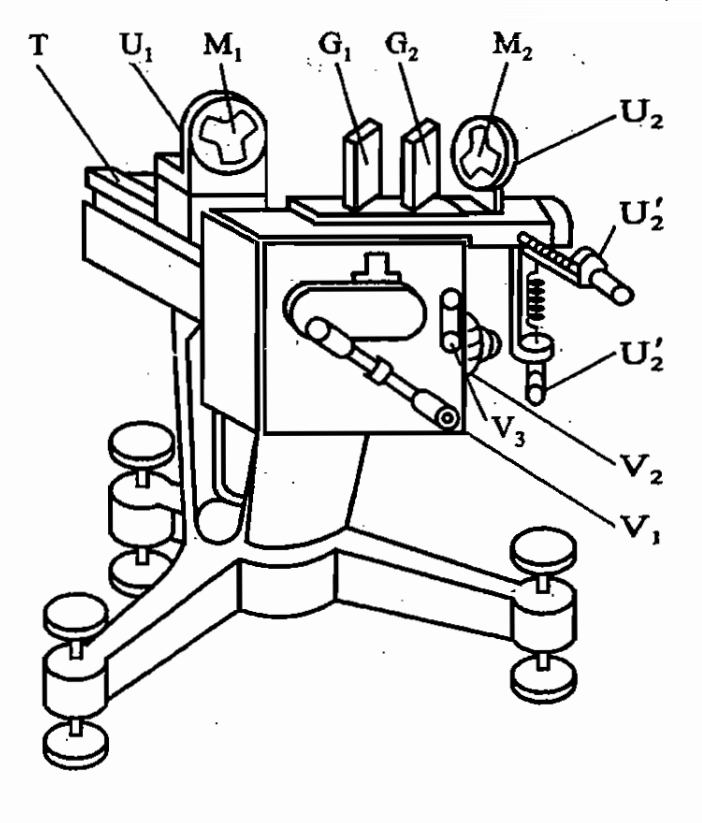
\includegraphics[width=5cm]{M.png}
		\caption{M-干涉仪}
	\end{figure}
\subsection*{【实验现象及描述】}

\subsubsection*{1.M-干涉仪的调节步骤}
	\begin{enumerate}[(1)]
	\item 调节氦氖激光器的高度.利用针孔盘前后移动确定激光器的高度是否合适.当针孔盘贴近激光器时,调节两者的高度使得激光恰好从孔中穿出;当针孔盘贴近M-干涉仪时,调节激光器的俯仰角与旋角使得激光从孔中穿出.
	\item 调整激光器与M-干涉仪的相对位置,将其摆正,使得激光照射到$G_1$的正中位置.
	\item 调节$M_1$和$M_2^{\prime}$的平行位置.观察激光器出射口位置的光点,使用$U_1$和$U_2$的粗调与细调,使得最亮的光点与出射口大致重合.
	\end{enumerate}
\subsubsection*{2.非定域干涉圆条纹的调节步骤}
	继上述步骤之后,我们只需要在激光器与分束板之间加一个显微物镜使得光束会聚成为点光源,此时在观察屏上便能观察到圆条纹,如图2所示.
	\begin{figure}[htbp]
	\centering
		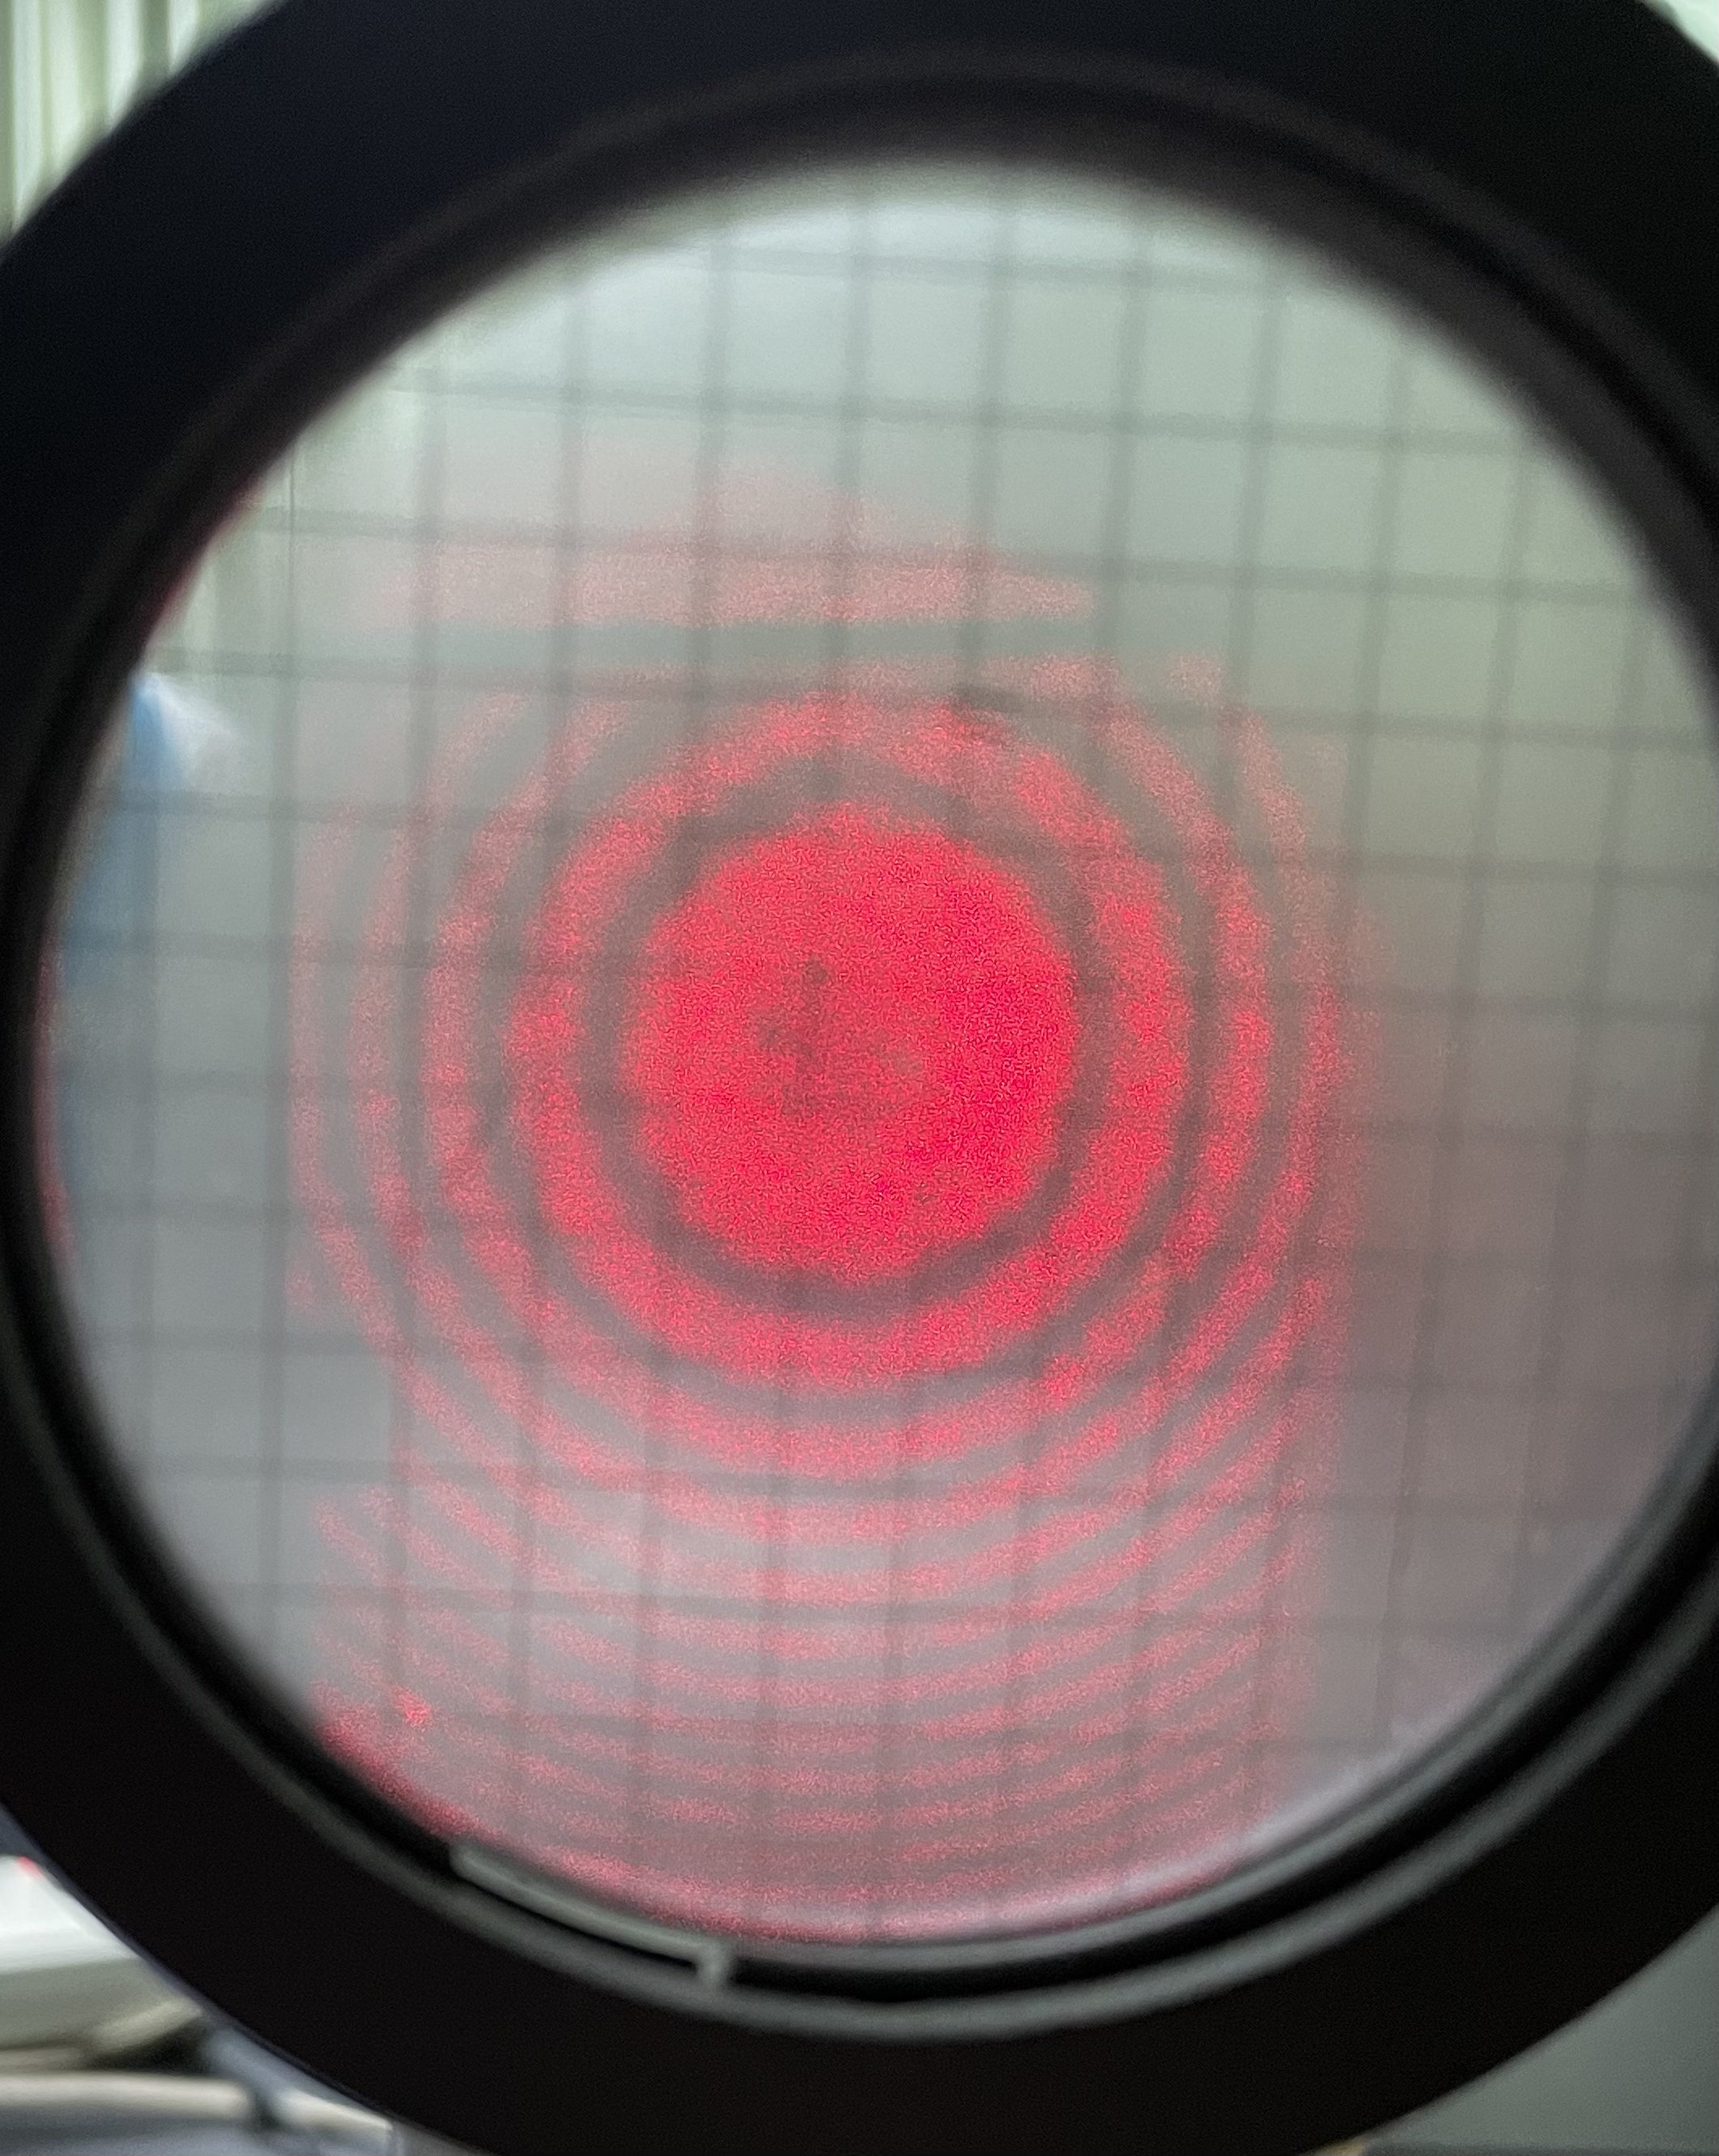
\includegraphics[width=4cm]{ganshe.jpg}
		\caption{非定域圆条纹}
	\end{figure}
	\newpage
	当然最开始放上观察屏时,看到的可能只是圆条纹的一部分,这表明圆心并没有在屏上,此时只需要调节$U_2^{\prime}$就能慢慢把圆心移到屏上.\par
	而对于椭圆条纹来说,只需要将观察屏倾斜一定角度即可.\par
	在观察圆条纹时,转动$M_1$使得$d$发生改变,会发现当$d$增加时,会发生条纹的“吐”,而当$d$减小时,会发生条纹的“吞”.当$d$增加时,条纹越来越密,且条纹也越来越窄,而且$r_k$也变大了,在扩张.\par
	下面是理论解释:
	\begin{figure}[htbp]
		\centering
		\subfloat[干涉场]{
				\label{fig:improved_subfig_a}
				\begin{minipage}{0.5\textwidth}
					\centering
					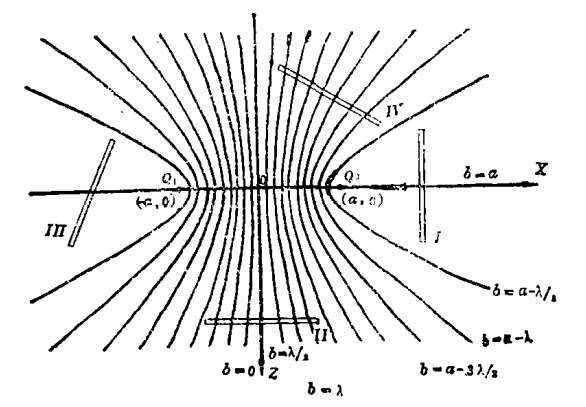
\includegraphics[height=10cm]{shuangquxian.png}
				\end{minipage}
		}
		\subfloat[非定域干涉原理]{
				\label{fig:improved_subfig_b}
				\begin{minipage}{0.5\textwidth}
					\centering
					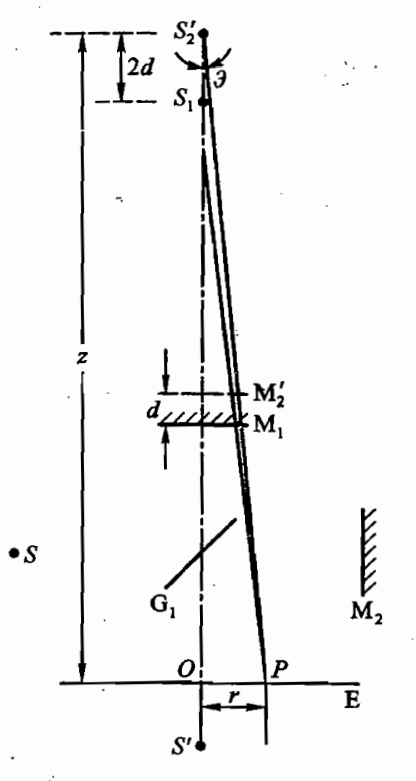
\includegraphics[height=10cm]{lilun.png}
				\end{minipage}
		}
		\caption{原理图}
	\end{figure}
	\par
	首先我们分析一下非定域干涉的特性,假设在$xz$平面上由相距为$2a$的两个相干点光源,如图3(a)所示.则该平面上任意一点的光强就是$I(p)=I_1+I_2+2\sqrt{I_1I_2}\cos(2\pi\dfrac{\Delta L}{\lambda})$,现在令$\Delta L=2b=\pm n\lambda$,则$\cos(2\pi\dfrac{\Delta L}{\lambda})=1$,此时光强达到最大值.而且该公式中的$\sqrt{I_1I_2}$也解决了为什么分束板的透射比接近1的问题,因为只有当透射比为1时,$\sqrt{I_1I_2}$才能最大,而干涉图样也能更加清晰. 又由于$\Delta L=|\sqrt{(x+a)^2+z^2}-\sqrt{(x-a)^2+z^2}|=2b$,则解出方程为$\dfrac{x^2}{b^2}-\dfrac{z^2}{a^2-b^2}=1$,说明同光强的干涉点在一条条双曲线的分支上.在$xz$平面上画出就如图3(a)所示,当观察屏与$x$轴垂直,也即与两相干点连线垂直时,由于空间对称性,干涉条纹便会是一个个同心圆.由于干涉场以$x$轴对称,则在三维空间中干涉点的方程为$\dfrac{x^2}{b^2}-\dfrac{y^2+z^2}{a^2-b^2}=1$,同时投射到屏上的同心圆半径为
	$$
	r=\sqrt{y^2+z^2}=\sqrt{(a^2-b^2)(\frac{c^2}{b^2}-1)}
	$$
	其中,$c$是投屏与$O$点之间的距离.该方程就是能出现圆条纹、椭圆条纹、直线条纹和双曲线条纹的理论依据.\par
	接下来分析圆条纹变化的原因.如图3(b)所示,由于$\theta$是小角度,那么就有$\cos\theta\approx1-\theta^2,\theta\approx r/z$,则有$\Delta L=2d(1-\dfrac{r^2}{2z^2})=k\lambda$.假设$r_k$和$r_{k-1}$,则$\Delta r=r_{k-1}-r_k\approx \dfrac{\lambda z^2}{2r_kd}$.则$d$越大,$\Delta r$越小,即圆条纹越密,也就越细;$d$越小,$\Delta r$越大,即圆条纹越疏,也就越粗.当$d$增大时,$r_k$会增大,所以会有“吐”条纹的情况;当$d$减小时。$r_k$会减小,所以会有“吞”条纹的情况.
\subsubsection*{3.非定域直条纹和双曲条纹的调节办法}
	如图3(a)所示,当观察屏垂直于$z$轴摆放,即在M-干涉仪实验中平行于$S_1$和$S_2^{\prime}$连线时,那么干涉点方程变换为
	$$
	\frac{x^2}{b^2}-\frac{y^2}{a^2-b^2}=1+\frac{c^2}{a^2-b^2}=const
	$$
	其中$c$是屏与$O$点的距离.根据双曲线方程的特性,可判定上述方程代表的曲线是双曲线.显然有$b \ll a \ll c$,则方程变化为$x^2=\dfrac{b^2c^2}{a^2}$,该方程明显是直线方程,又$2b=n\lambda$,则可得直线间距为$\dfrac{c}{2a}\lambda$.因此我们看到的直线并不是真正的直线,而是双曲线近似而来的.那么如果我们要观察双曲条纹,只需要加强一些双曲线的特性即可,比如在观察到直线条纹的位置,将观察屏旋转一个轻微的角度.
\subsubsection*{4.定域干涉的调节}
\textcircled{1}等倾干涉:\\
在非定域干涉的调节基础之上,去掉显微物镜,放上毛玻璃散射屏使光束散射成为扩展光源,因为等倾干涉需要不同入射角的光束.\\
当移动$M_1$使$d$增加时,由于$\Delta L=2d=n\lambda$,则圆心处的干涉级次越来越高,会看到条纹的“吐”,相应地当$d$减小时,会看到圆条纹的“吞”.\par
\textcircled{2}等厚干涉:\\
在等倾干涉的调节基础之上,调节$U_2$,调整$M_2$的角度,使得$M_1$和$M_2^{\prime}$之间形成一个非常小的角度,便于形成等厚干涉.若圆心并未在中心,需要调节$U_2^{\prime}$使得圆心出现视野中央.\\
由于是小角度,则$\Delta L \approx 2d\cos\theta \approx 2d(1-\theta^2/2)$.调整$V_1$,移动$M_1$,使得视野中的干涉条纹逐渐从弯曲变直再变弯曲,观察到该现象之后,将白炽灯打开,并将其对准散射屏.再调节$V_1$使条纹重新回到弯曲状态,再使用$V_2$细调,缓慢转动$V_2$,最后会找到如图4所示的彩色干涉条纹.而此时的$d_0=50.73750(mm)$.
\begin{figure}[htbp]
		\centering
		\subfloat[远视角]{
				\label{fig:improved_subfig_a}
				\begin{minipage}{0.5\textwidth}
					\centering
					\includegraphics[width=8cm,angle=270]{caise1.jpg}
				\end{minipage}
		}
		\subfloat[近视角]{
				\label{fig:improved_subfig_b}
				\begin{minipage}{0.5\textwidth}
					\centering
					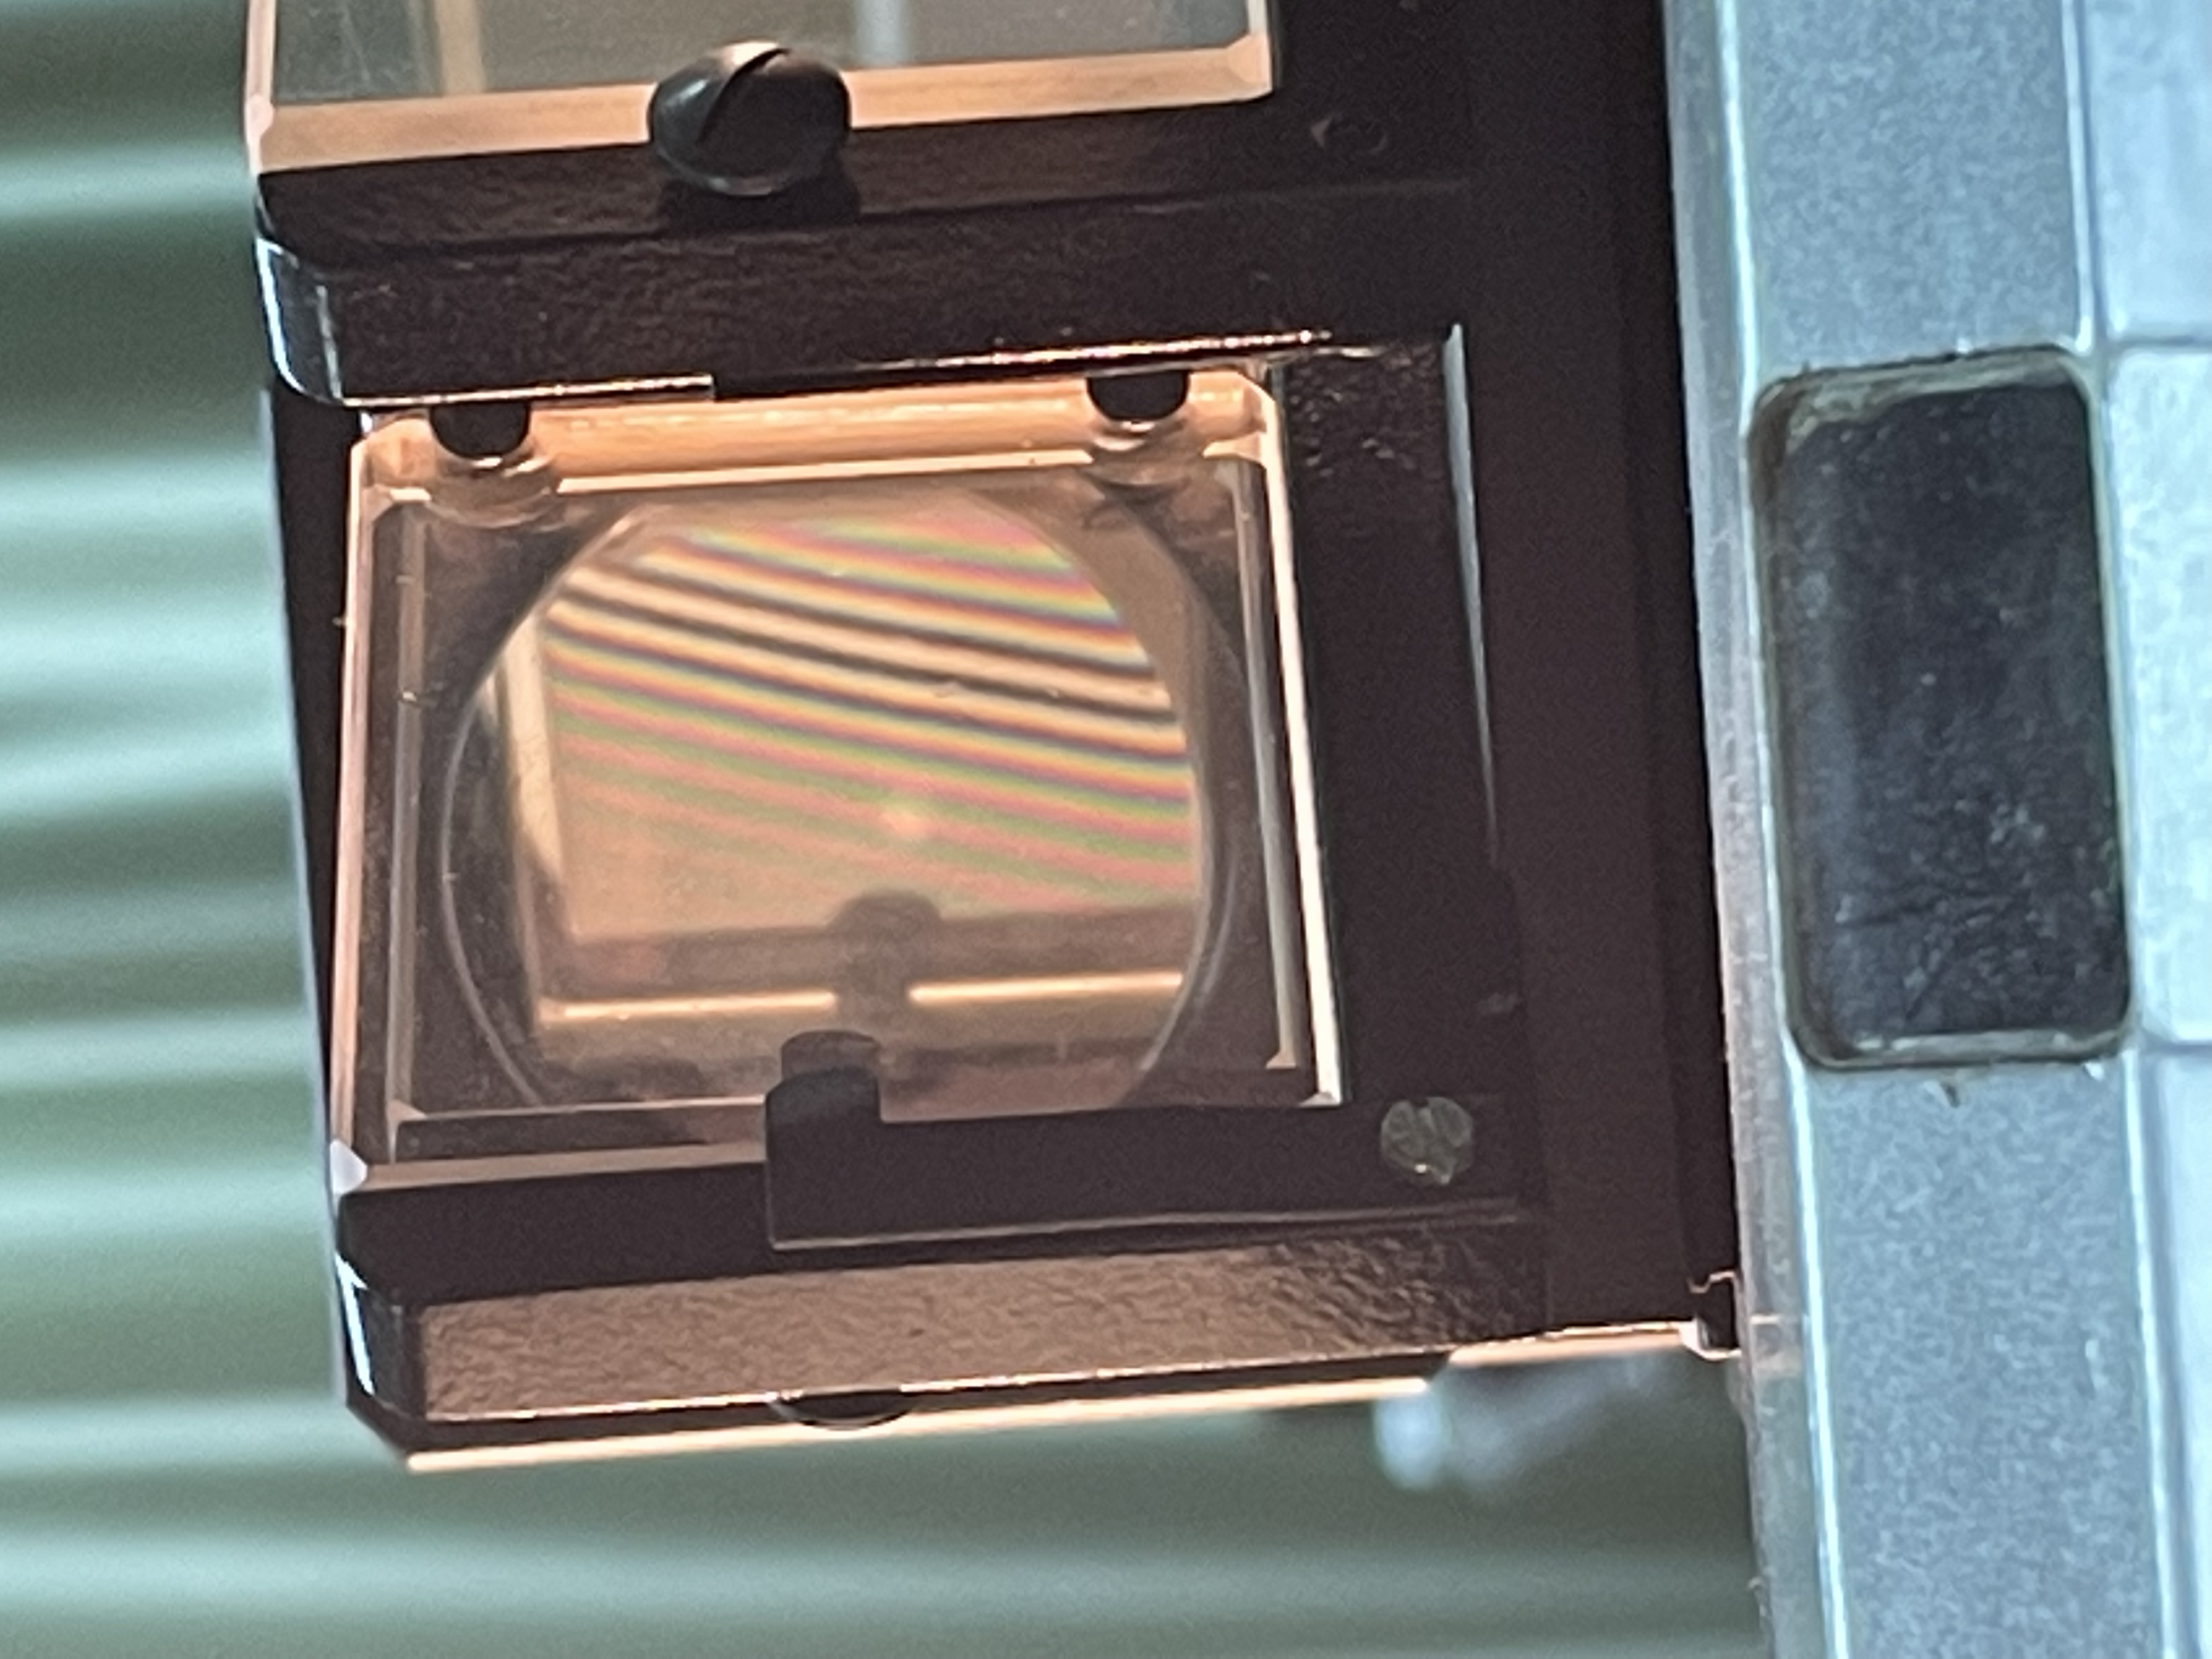
\includegraphics[width=8cm,angle=270]{caise2.jpg}
				\end{minipage}
		}
		\caption{白光干涉图样}
	\end{figure}
\subsection*{【压电陶瓷的压电常量的测量 】}	
已知条件为:$L=46mm\quad t=1.0mm\quad\lambda=632.8mm$\par
下表为从某一状态开始,每“吐”一个圆条纹时记录的电压值.\par
\begin{table}[htbp]
\centering
\scalebox{1.3}{
\begin{tabular}{cccccccccc}
\hline\hline
$n$&0&1&2&3&4&5&6&7&8 \\
\hline
$U_f/V$&-150.8&-122.9&-95.6&-69.5&-48.2&-31.4&-6.3&16.2&35.2 \\
\hline
\end{tabular}}
\end{table}
经过matlab的回归计算,得出斜率为$22.9667$.又因为斜率代表$\dfrac{\lambda t}{2d_{21}L}$,则有$d_{21}=\dfrac{632.8\times1.0}{2\times46\times22.9667}\approx 0.3(mm/V)$	.\\
\newpage
下面是经过matlab画出的线性回归图:
\begin{figure}[htbp]
\centering
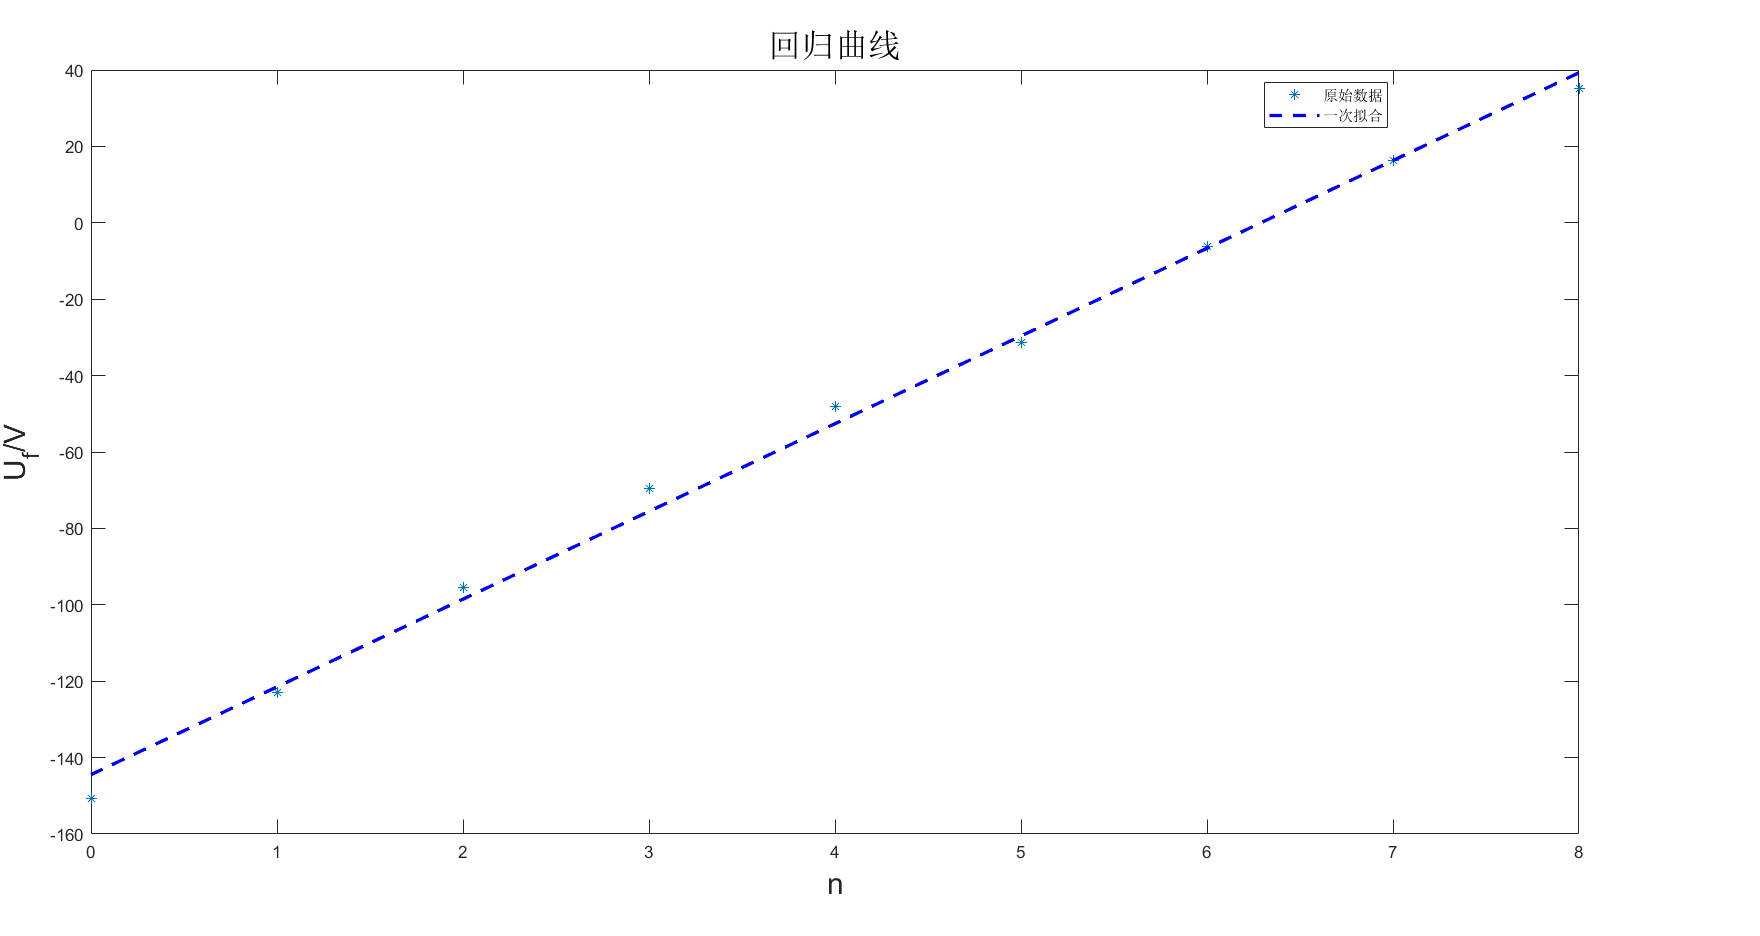
\includegraphics[width=18cm]{huigui.png}
\caption{压电陶瓷线性回归图}
\end{figure}
\subsection*{【分析与讨论】}
\begin{enumerate}[(1)]
\item 在测量压电陶瓷的压电常量时,需要观察圆条纹的“吞吐”现象,但是对于圆来说,从开始吐直到吐出一个完整的圆条纹,其间是比较难以把握的,该测量误差对最后的压电常数会造成一些误差.
\item 当等倾干涉条纹完全是圆形时,此时可以判断$M_1$和$M_2^{\prime}$平行度极高,即干涉条纹越圆,平行度越高.
\end{enumerate}
\subsection*{【收获与感想】}
M-干涉仪是为了研究“以太”的存在而创造的仪器,最后否定了“以太”的存在论,为狭义相对论提供了实验上的依据.如今,这件精细的仪器依然在物理领域散发着光芒——在引力波探测中发挥着巨大作用,同时M-干涉仪的原理也运用在了LISA中,为宇宙探索尽了一份力,再一次感慨迈克尔逊和莫雷的伟大!
\newpage
\subsection*{【参考文献】}
[1]陈怀琳.迈克耳孙干涉仪所产生的非定域干涉条纹.物理实验,1983(5):200 \par
[2]尤德红.迈克尔逊干涉仪椭圆干涉图样成因分析[J]. 技术物理教学, 2008, 16(3)
	
	
	
	
\end{document}